\subsection{Ca sử dụng chỉnh sửa thông tin cá nhân}
\vspace{0.5cm}


\noindent 
\begin{tabularx}{\linewidth}{| l | X |} 
\hline 
\textbf{Mô tả} & Người dùng cập nhật thông tin cá nhân như
địa chỉ, tên, số điện thoại, mô tả, ảnh đại diện,v.v. \\ 
\hline 
\textbf{Luồng cơ bản} & 1. Người dùng truy cập tab tài khoản và bấm vào trang hồ sơ của bản thân \newline
                       2. Người dùng ấn vào nút chính sửa \newline
                       3. Người dùng nhập các thông tin cần thay đổi. \newline
                       5. Người dùng ấn nút submit. \newline
                       6. Hệ thống cập nhật thông tin người dùng và thông báo cập nhật thành công. \\
\hline 
\textbf{Luồng thay thế} & Nếu Người dùng nhập thông tin không hợp lệ hệ thống sẽ báo lỗi. \\
\hline 
\textbf{Tiền điều kiện} & Người dùng đang đăng nhập và phiên đăng nhập chưa kết thúc. \\
\hline 
\textbf{Hậu điều kiện} & Thông tin mới của người dùng được cập nhật. \\

\hline 
\textbf{Yêu cầu phi chức năng} & Hệ thống xử lý cập nhật không quá 5s (do có upload ảnh) \\ 
\hline 
\end{tabularx}

\vspace{0.8cm}

\noindent 
\begin{tabular}{| c | c |}
    \hline
    \textbf{Biểu đồ hoạt động} & \textbf{Quan hệ} \\ 
    \hline
    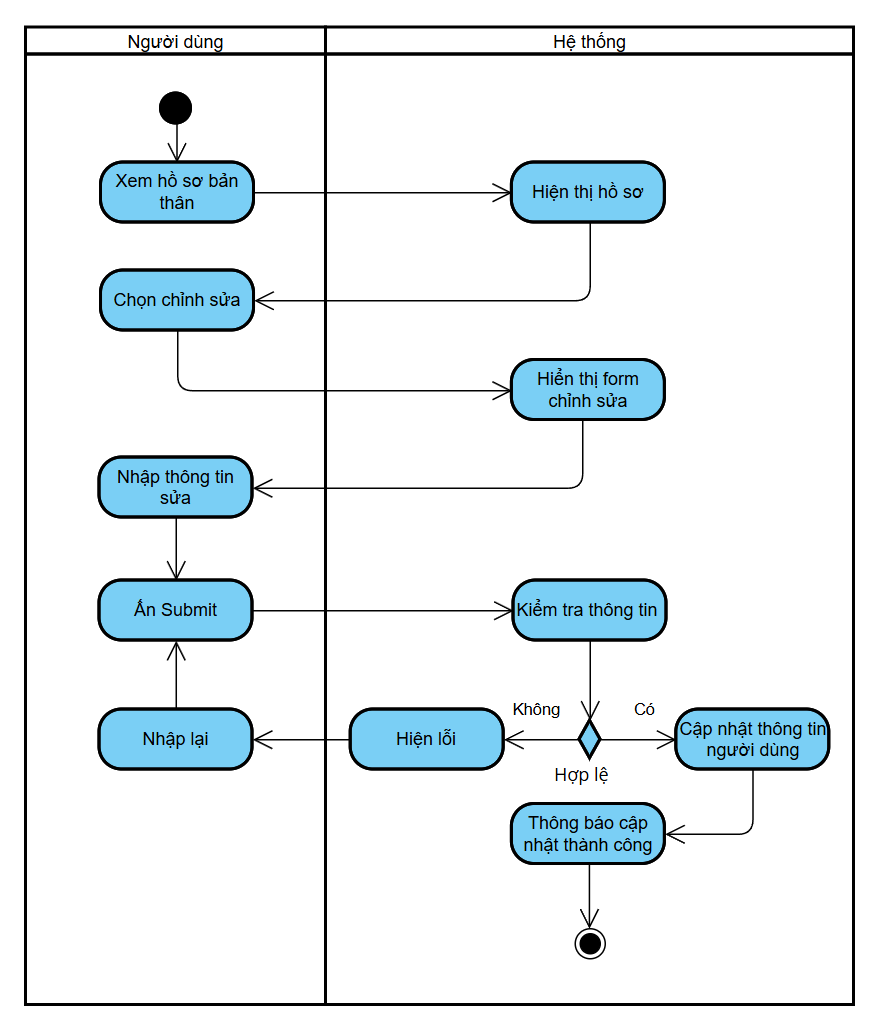
\includegraphics[width=0.5\linewidth]{figures/c3/3-3-4-ad.png} 
    & 
    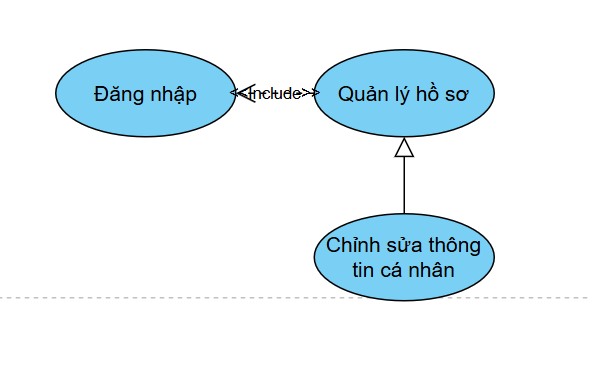
\includegraphics[width=0.45\linewidth]{figures/c3/3-3-4-rd.png} \\ 
    \hline
\end{tabular}



\begin{figure}[H]
    \centering  
    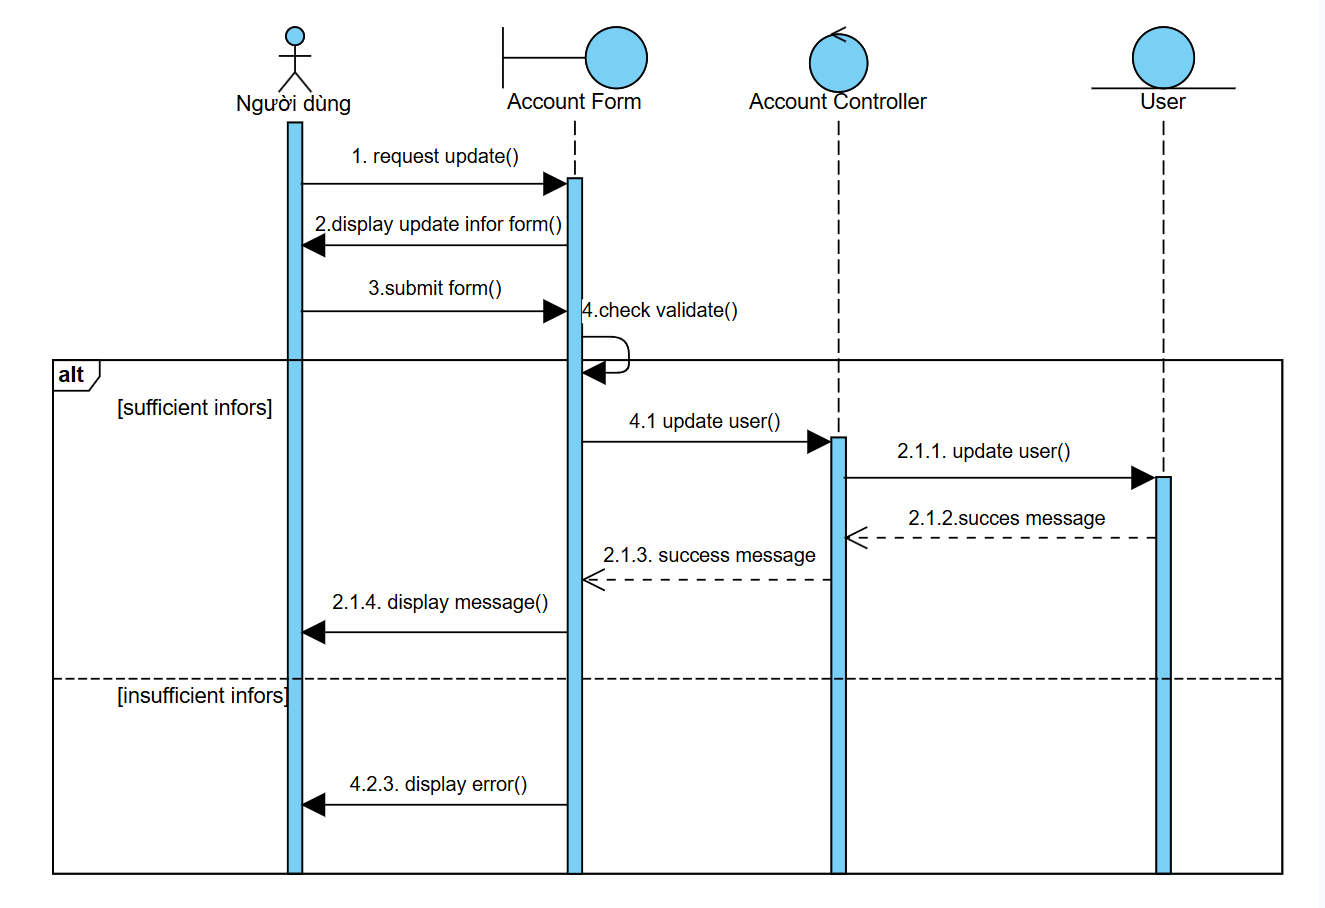
\includegraphics[width=1\textwidth]{figures/c3/3-3-4-sd.png}
    \caption{Biểu đồ tuần tự ca sử dụng chỉnh sửa thông tin cá nhân.}
    \label{fig:3-3-4-sequence-diagram}
\end{figure}